\documentclass{article}
\usepackage[margin=1.0in]{geometry}
\usepackage{amsmath, amssymb, mathrsfs}
\usepackage[english]{babel}
\usepackage{graphicx}
\usepackage{enumerate}
\usepackage{tikz}
\usetikzlibrary{shapes,backgrounds}

\title{Numerical Computing HW 6}
\author{Greg Stewart}
\date{\today}

\begin{document}

\maketitle

\section*{7.1(a)  \normalsize Derive a $O(k^2)$ approximation of $y'(t_j)$ that uses $y(t_j), y(t_{j-1}), y(t_{j+2})$.}

We need something of the form

$$y'(t_j) = ay(t_{j-1}) + by(t_j) + cy(t_{j+2})$$

Taylor expansions of the first and third terms in this expression are helpful:

$$y(t_{j-1}) = y(t_j-k) = y_j -ky_j' + \frac{k^2}{2}y_j'' + \cdots$$
$$y(t_{j+2}) = y(t_j+2k) = y_j + 2ky_j' + 2k^2y_j'' + \cdots$$

To solve for the coefficients $a$, $b$, and $c$, we can set up a system of equations using the taylor expansions:

$$(a + b + c)y_j = 0$$
$$(-a + 2c)ky_j' = y_j' \implies (2c - a)k = 1$$
$$(\frac{1}{2}a + 2b)k^2y_j'' = 0$$

Solving for the coefficients, we have

\begin{align*}
  a &= -4c \\
  b &= \frac{1}{6k} \\
  c &= \frac{1}{2k} \\
\end{align*}

So finally we have the finite difference equation

$$y'(t_j) = -\frac{2}{3k}y_{j-1} + \frac{1}{2k}y_j + \frac{1}{6k}y_{j+2}$$ 




\section*{7.5  \normalsize}

\textit{The shear stress $S(x)$ for a power law fluid is $$S=\alpha\Big(\frac{dv}{dx}\Big)^{\gamma}$$ where $v(x)$ is the shear velocity, and $\alpha$ and $\gamma$ are positive constants. You can assume the fluid is ketchup at room temperature, so $\gamma = \frac{1}{4}$ and $\alpha = 20$. Using second-order approximations for $v'(x)$, and the data in the table, find $S$ at $x = 0, \frac{1}{3}, \frac{2}{3}, 1$.}

\begin{table}[h!]
  \centering
  \begin{tabular} {c | c c c c c }
    $x$ & 0 & $\frac{1}{3}$ & $\frac{2}{3}$ & 1 \\ 
    \hline  
    $v$ & 0 & 2 & 4 & 0 \\
  \end{tabular}
\end{table}

We can start off by writing the equation out with the given values of $\alpha$ and $\gamma$:

$$S = 20(v'(x))^{\frac{1}{4}}$$

We can use the one-sided difference approximation to get all the values of S that we need. Note $k = \frac{1}{3}$.

\begin{align*}
  S(0) &= 20\cdot\Big(\frac{-v(2/3) + 4v(1/3) - 3(v(0))}{2/3}\Big)^{1/4} \\
  &= 20 \cdot \Big(\frac{-4 + 8}{2/3}\Big)^{1/4} \\
  &= 20(6)^{1/4} \\
  S(1/3) &= 20\cdot\Big(\frac{0 + 16 - 6}{2/3}\Big)^{1/4} \\
  &= 20(15)^{1/4} \\
  S(2/3) &= 20\cdot\Big(\frac{3v(2/3) - 4v(1/3) + v(0)}{2/3}\Big)^{1/4} \\
  &= 20 \cdot \Big(\frac{12 - 8}{2/3}\Big)^{1/4} \\
  &= 20(6)^{1/4} \\
  S(1) &= 20\cdot\Big(\frac{-16 + 2}{2/3}\Big)^{1/4} \\
  &= 20(-21)^{1/4}
\end{align*}

Now we can put this into a table.

\begin{table}[h!]
  \centering
  \begin{tabular} {c | c c c c c }
    $x$ & 0 & $\frac{1}{3}$ & $\frac{2}{3}$ & 1 \\ 
    \hline  
    $S$ & 31.302 & 39.360 & 31.302 & 30.274(1+i) \\
  \end{tabular}
\end{table}



\section*{7.6(b)  \normalsize The Bernoulli equation is}

$$y' + y^3 = \frac{y}{1+t}$$

\begin{enumerate}[(a)]\setcounter{enumi}{1}
  \item \textit{If the trapezoidal method is used to solve the equation, what is the resulting finite difference equation?}

    In this case, we have

    $$f(t, y) = \frac{y}{1+t} - y^3$$

    and the trapezoidal finite difference equation is

    $$y_{j+1} = y_j + \frac{k}{2}(f_j + f_{j+1})$$

    so for the Bernoulli equation, we get the finite difference equation

    $$y_{j+1} = y_j + \frac{k}{2}\Big(\frac{y_j}{1+t_j} - y_j^3 + \frac{y_{j+1}}{1 + t_{j+1}} - y_{j+1}^3\Big)$$
\end{enumerate}






\section*{7.19  \normalsize}

\textit{Suppose you're computing the solution to $y' = e^{-y} + t^5$ for $0 \leq t \leq 1$ using 100 time steps. The methods to be used are Euler method, backward Euler method, trapezoidal mehtod, Heun, and RK4 method.}

\begin{enumerate}[(a)]
  \item \textit{Which one would you expect to complete the calculation the fastest?}

    Euler method should finish the calculation the fastest as it does the fewest total calculations---far fewer than any of the other methods.
  \item \textit{Which one would you expect to be the most accurate?}

    RK4 method should end up being the most accurate. It has the greatest reduction in error in relation to number of steps, and thus at 100 time steps should have the lowest error, making it the most accurate.
  \item \textit{If stability is a concern which method would be best?}

    Trapezoidal would be best if stability is a major concern. While implicit, it is A-stable, whereas most of the other methods are conditionally A-stable. As there are no conditions on the trapezoidal method's stability, and since it has better error than backward Euler method, it is the right choice as the most stable.
\end{enumerate}






\section*{7.21  \normalsize}

\textit{Solve the IVP involving the Bernoulli equation using trapezoidal and RK4 methods.}

$$y' + y^3 = \frac{y}{\alpha+t} \qquad t > 0 \qquad y(0) = 1$$

\begin{enumerate}[(a)]
  \item \textit{Verify the following exact solution and solve for $\beta$ from the IC.}

    $$y = \frac{\alpha + t}{\sqrt{\beta + \frac{2}{3}(\alpha + t)^3}}$$

    To do this we first rearrange the equation a bit, then apply the integrating factor method.

    \begin{align*}
      y' - \frac{1}{\alpha + t}y &= -y^3 \\
      y^{-3}y' - \frac{1}{\alpha + t}y^{-2} &= -1 \\
    \end{align*}
    
    Now let $v = y^{-2}$ so $v' = -2y^{-3}y'$ and make the appropriate substitutions.

    \begin{align*}
      -\frac{1}{2}v' - \frac{1}{\alpha + t}v &= -1 \\
      v' + \frac{2}{\alpha + t}v &= 2
    \end{align*}

    Let 

    $$\mu(x) = e^{\int\frac{2}{\alpha+t}dt} = (\alpha + t)^2$$

    and multiply across the equation.

    \begin{align*}
      (\alpha + t)^2v' + 2(\alpha + t)v &= 2(\alpha + t)^2 \\
      (\alpha + t)^2v' + \frac{d}{dt}\big[(a+t)^2\big]v &= 2(\alpha + t)^2 \\
      \int\frac{d}{dt}\big[(\alpha + t)^2v]dt &= \int2(\alpha + t)^2dt \\
      (\alpha + t)^2v &= \frac{2}{3}(\alpha + t)^3 + \beta \\
      v &= \frac{\frac{2}{3}(\alpha + t)^3 + \beta}{(\alpha + t)^2} \\
    \end{align*}

    Now we can substitute $v = y^{-2}$ and solve easily for $y$:

    $$y = \frac{\alpha + t}{\sqrt{\frac{2}{3}(\alpha + t)^3 + \beta}}$$

    Which is precisely what we wanted. Now, since $y(0) = 1$, we can solve for $\beta$:

    \begin{align*}
      1 &= \frac{\alpha}{\sqrt{\frac{2}{3}\alpha^3 + \beta}} \\
      1 &= \frac{\alpha^2}{\frac{2}{3}\alpha^3 + \beta} \\
      \beta + \frac{2}{3}\alpha^3 &= \alpha^2 \\
      \beta &= \alpha^2(1 - \frac{2}{3}\alpha)
    \end{align*}

  \item \textit{Assuming $\alpha = 0.01$, on the same axes plot the exact and the two numerical solutions for $0 \leq t \leq 3$ in the case of when $M=80$.}

    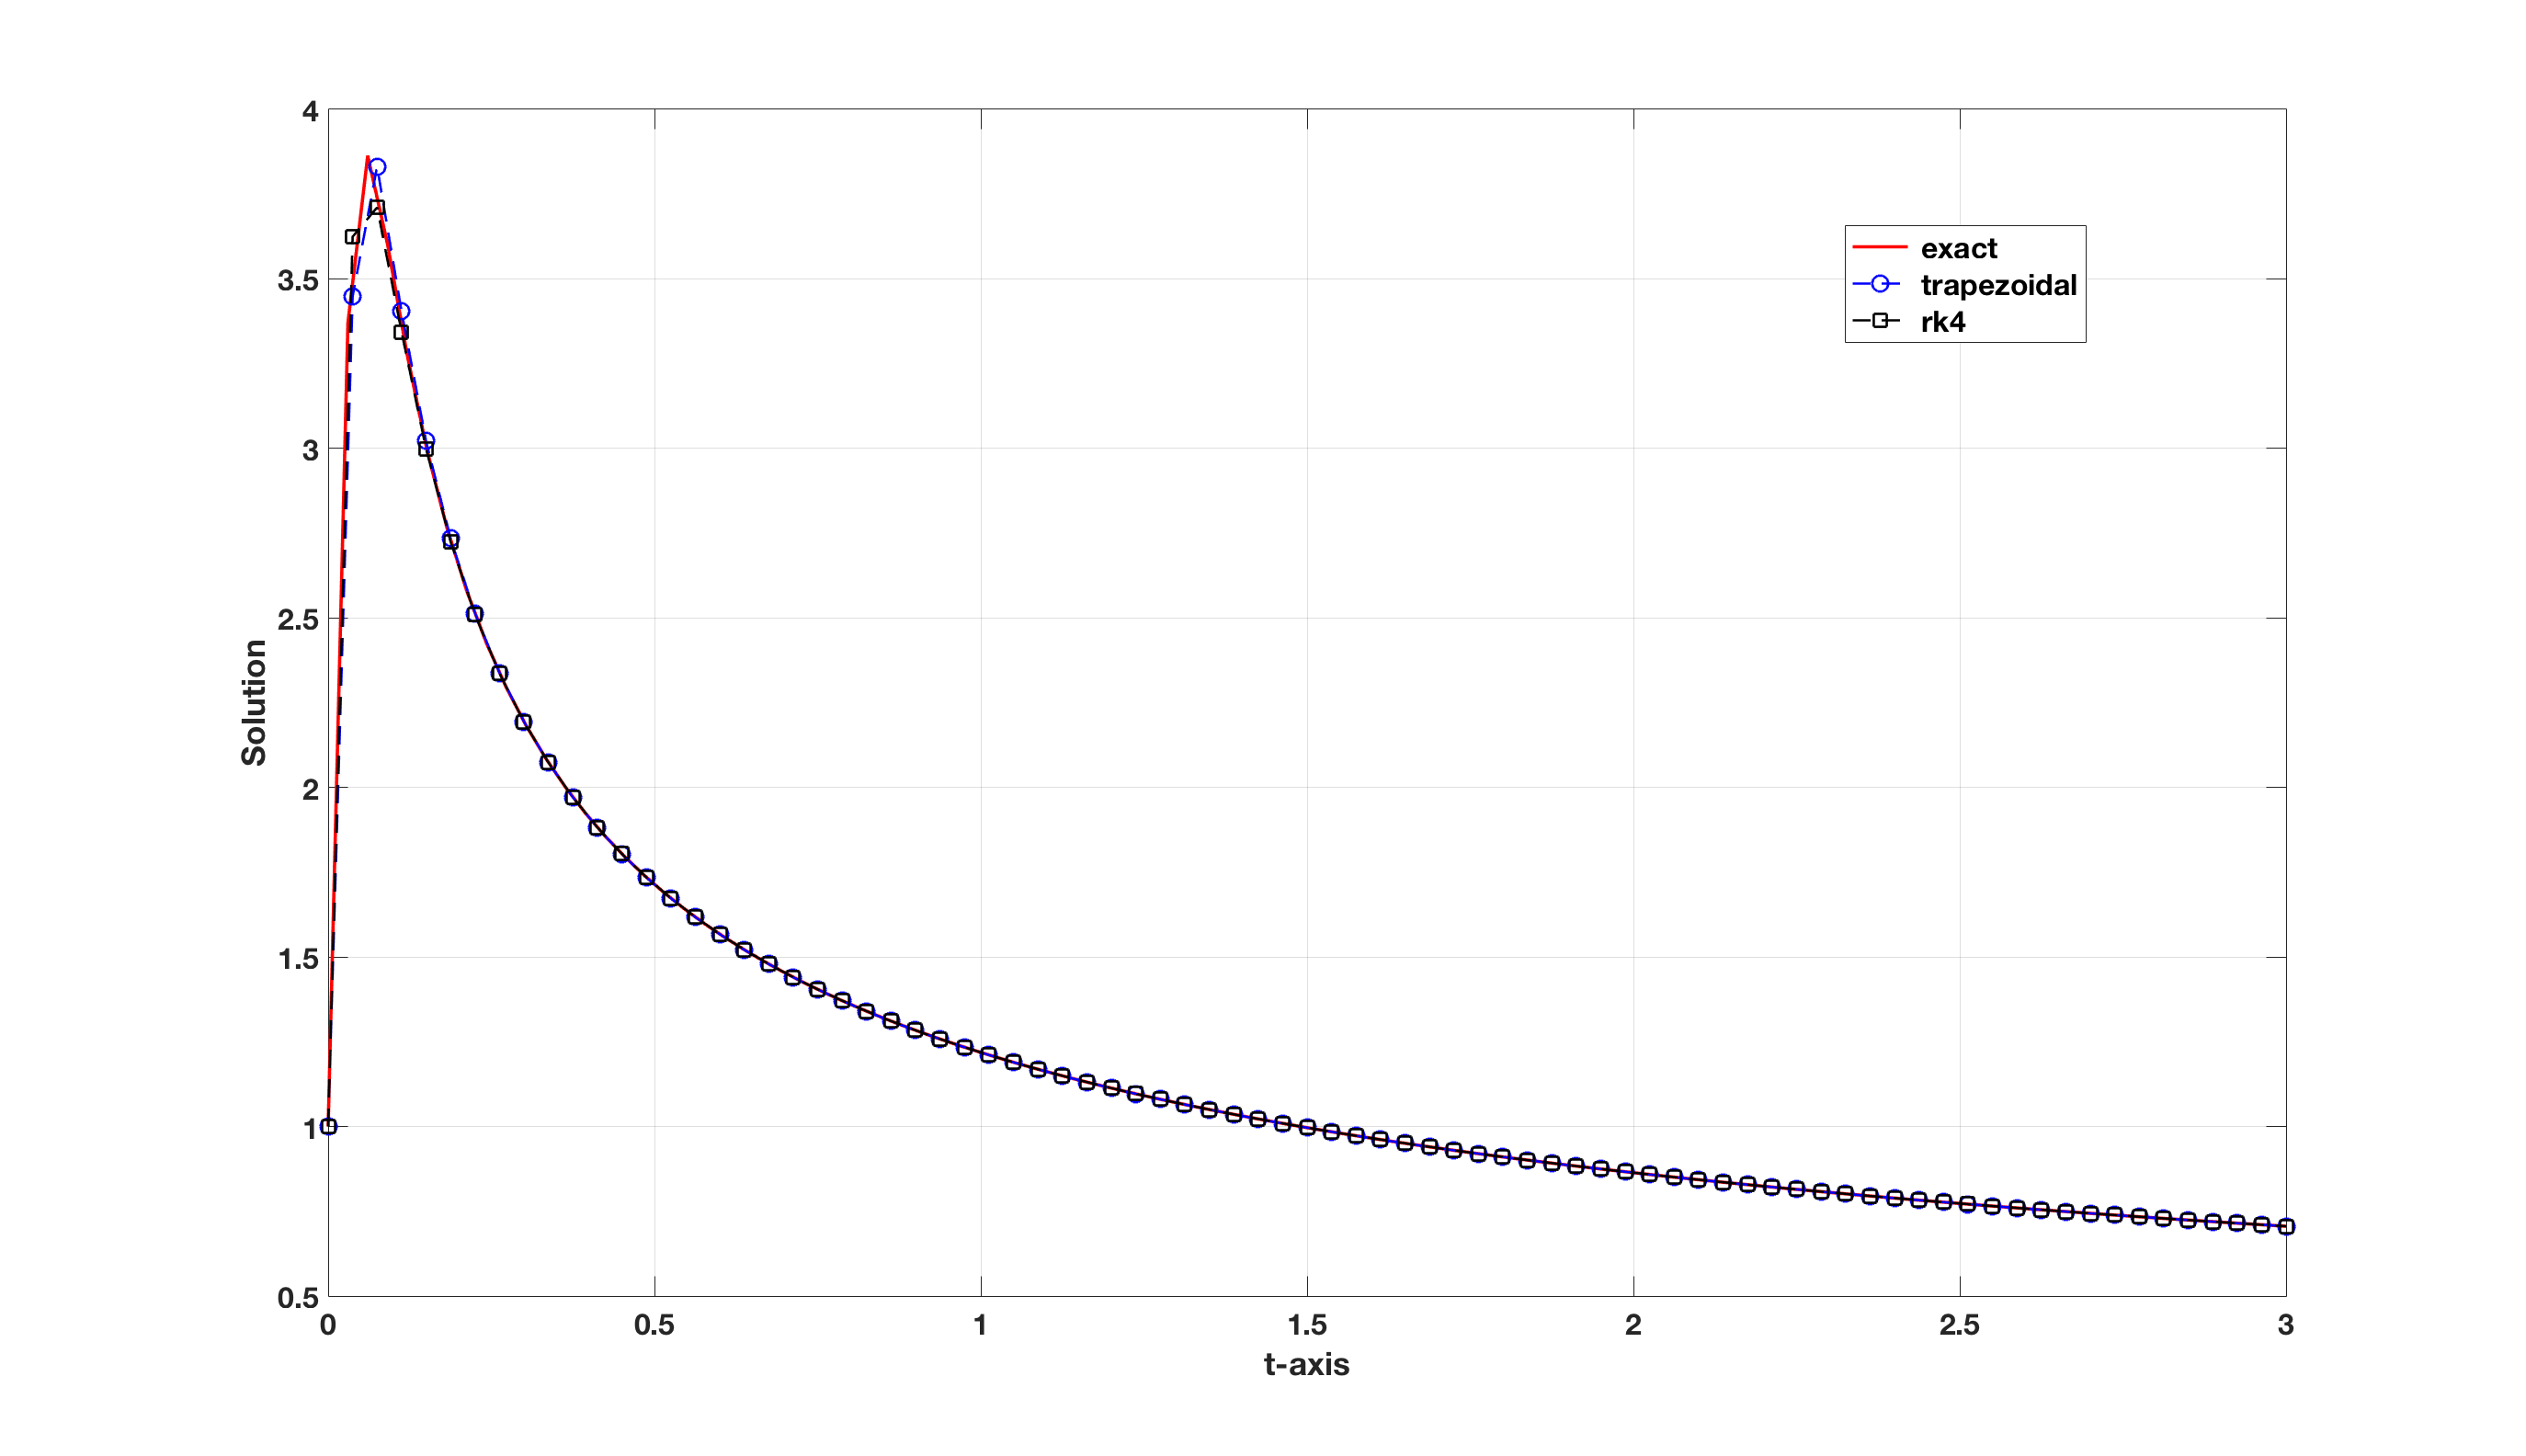
\includegraphics[width=\textwidth]{b.png}

  \item \textit{Redo (b) for $M=20,40,160$, with one graph for $M$. If one of the methods is unstable it can be excluded.}

    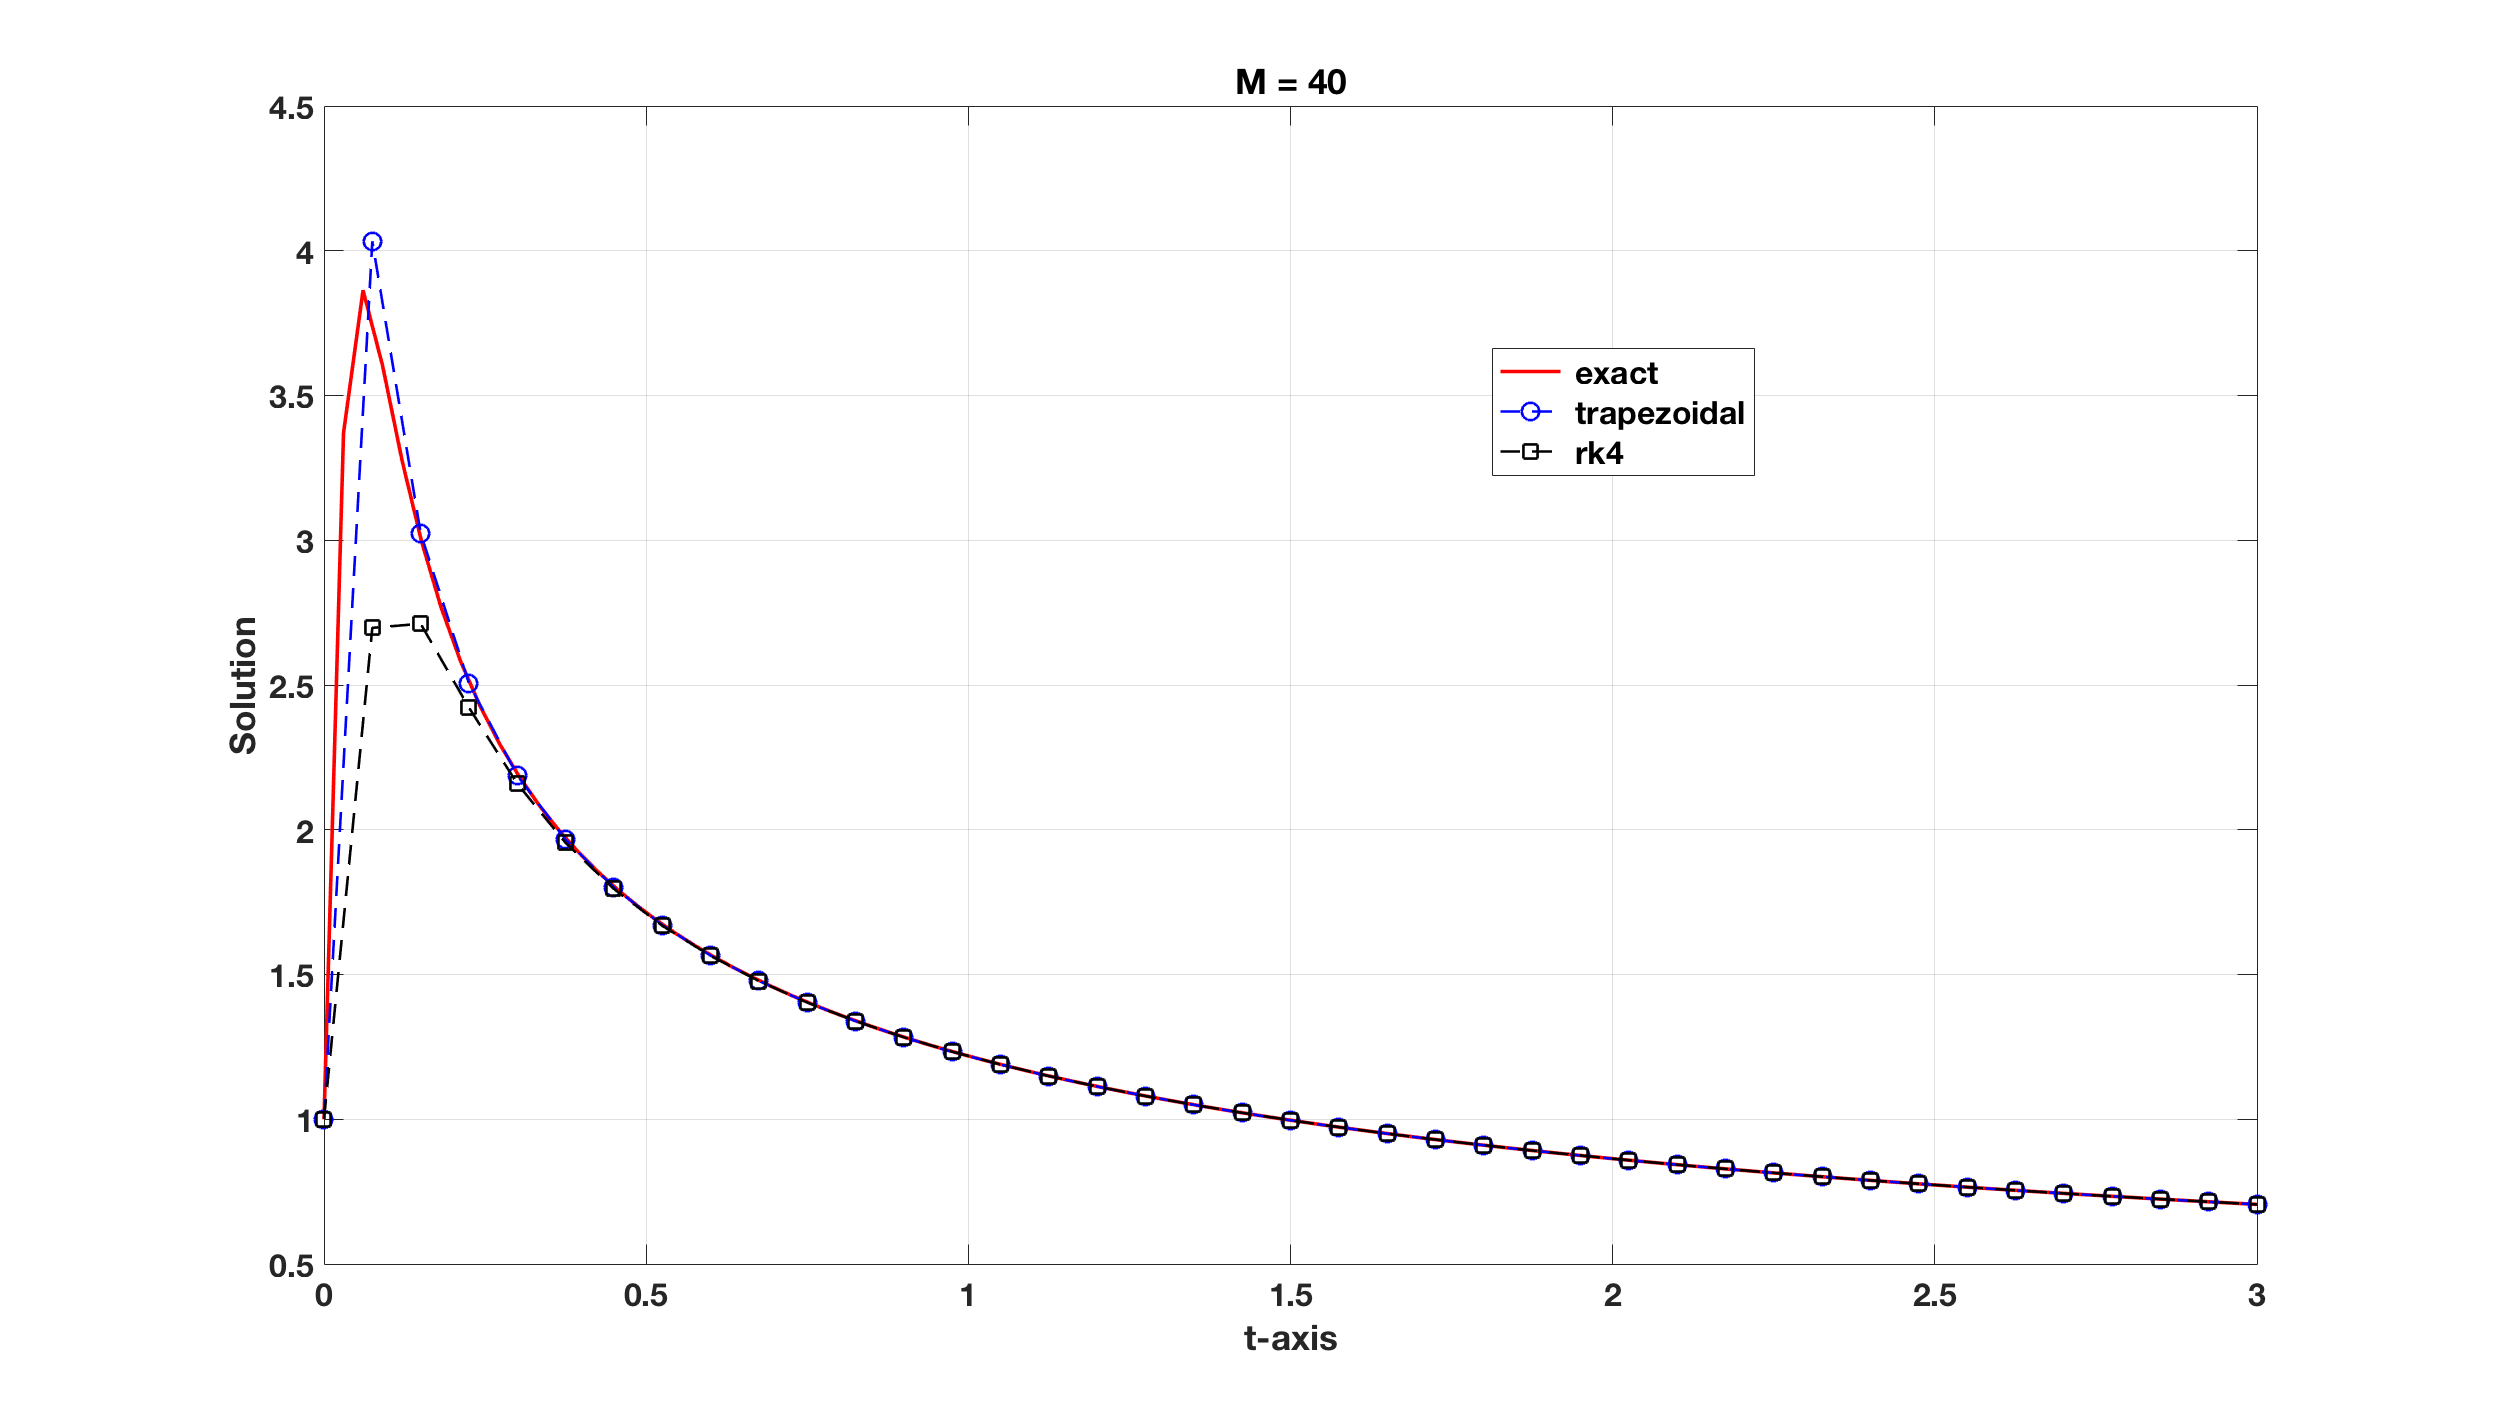
\includegraphics[width=\textwidth]{c40.png}

    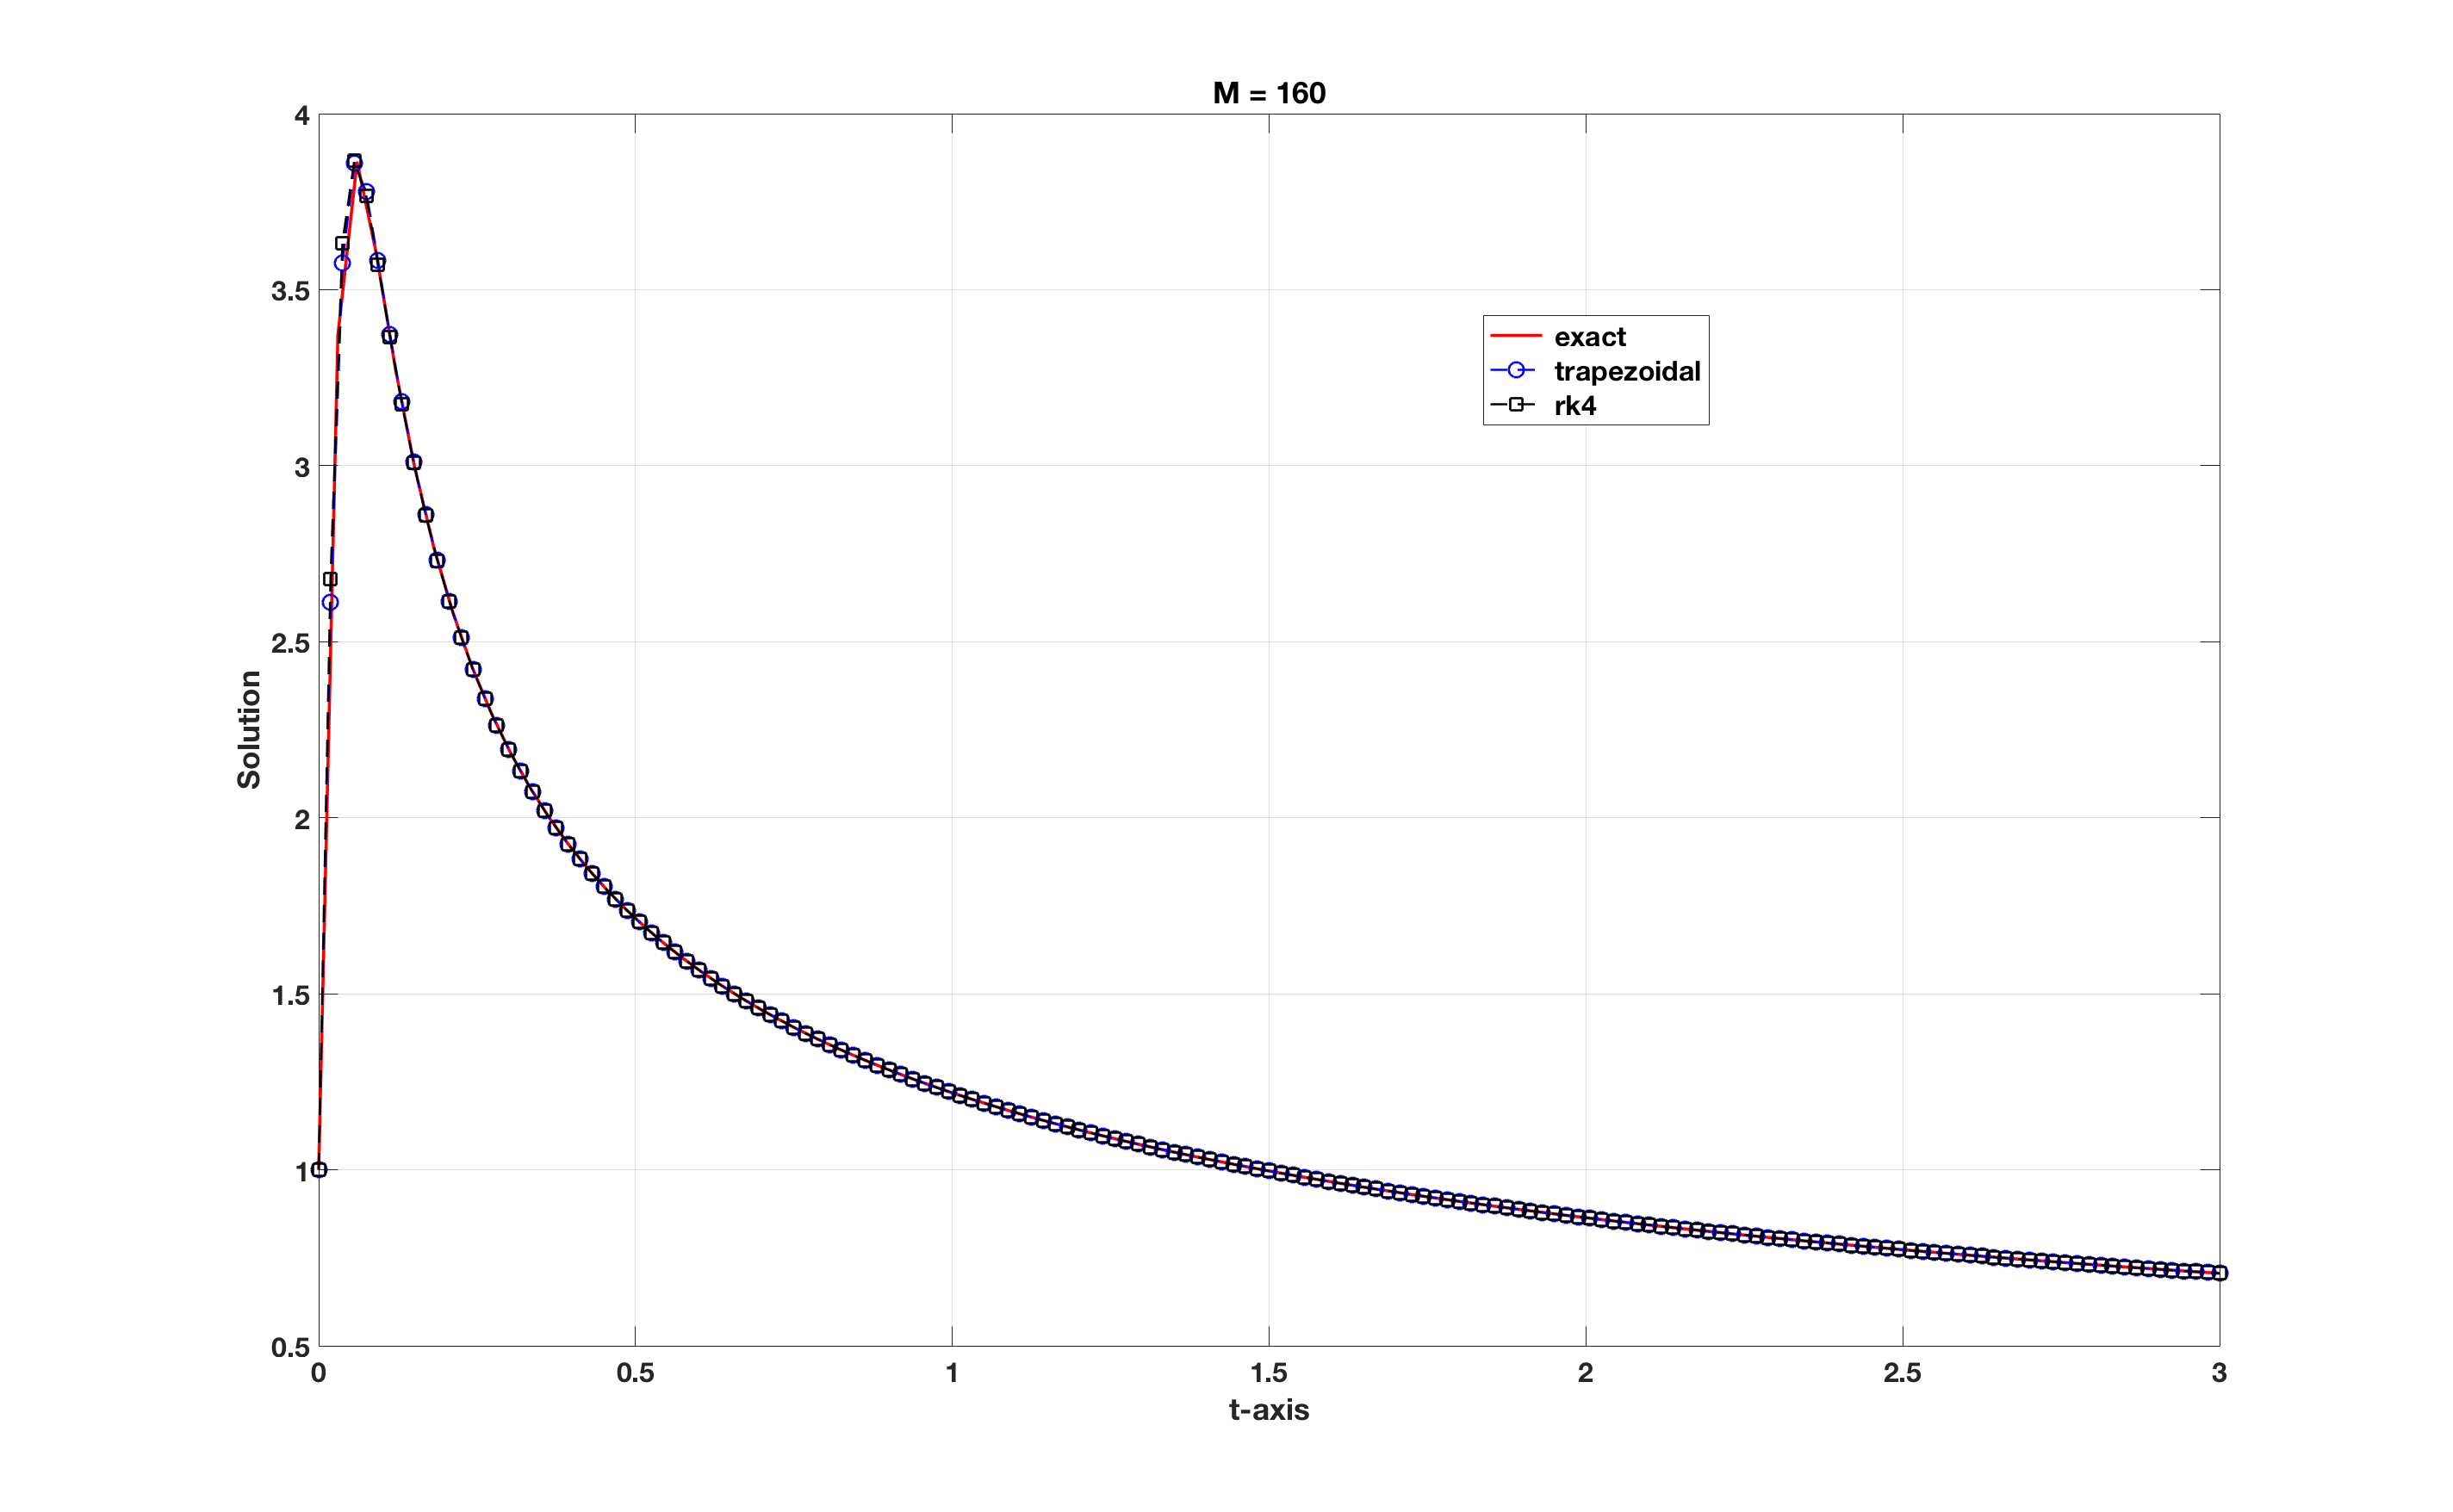
\includegraphics[width=\textwidth]{c160.png}

    \textbf{The plot for $M = 20$ was unstable for the RK4 method, and thus could not be plotted.}



  \item \textit{Plot the max error $e_{\infty}$ as a function $M$ for each method, using $M = 40,80,160,320,640$. The two curves should be in the same log-log plot.}

    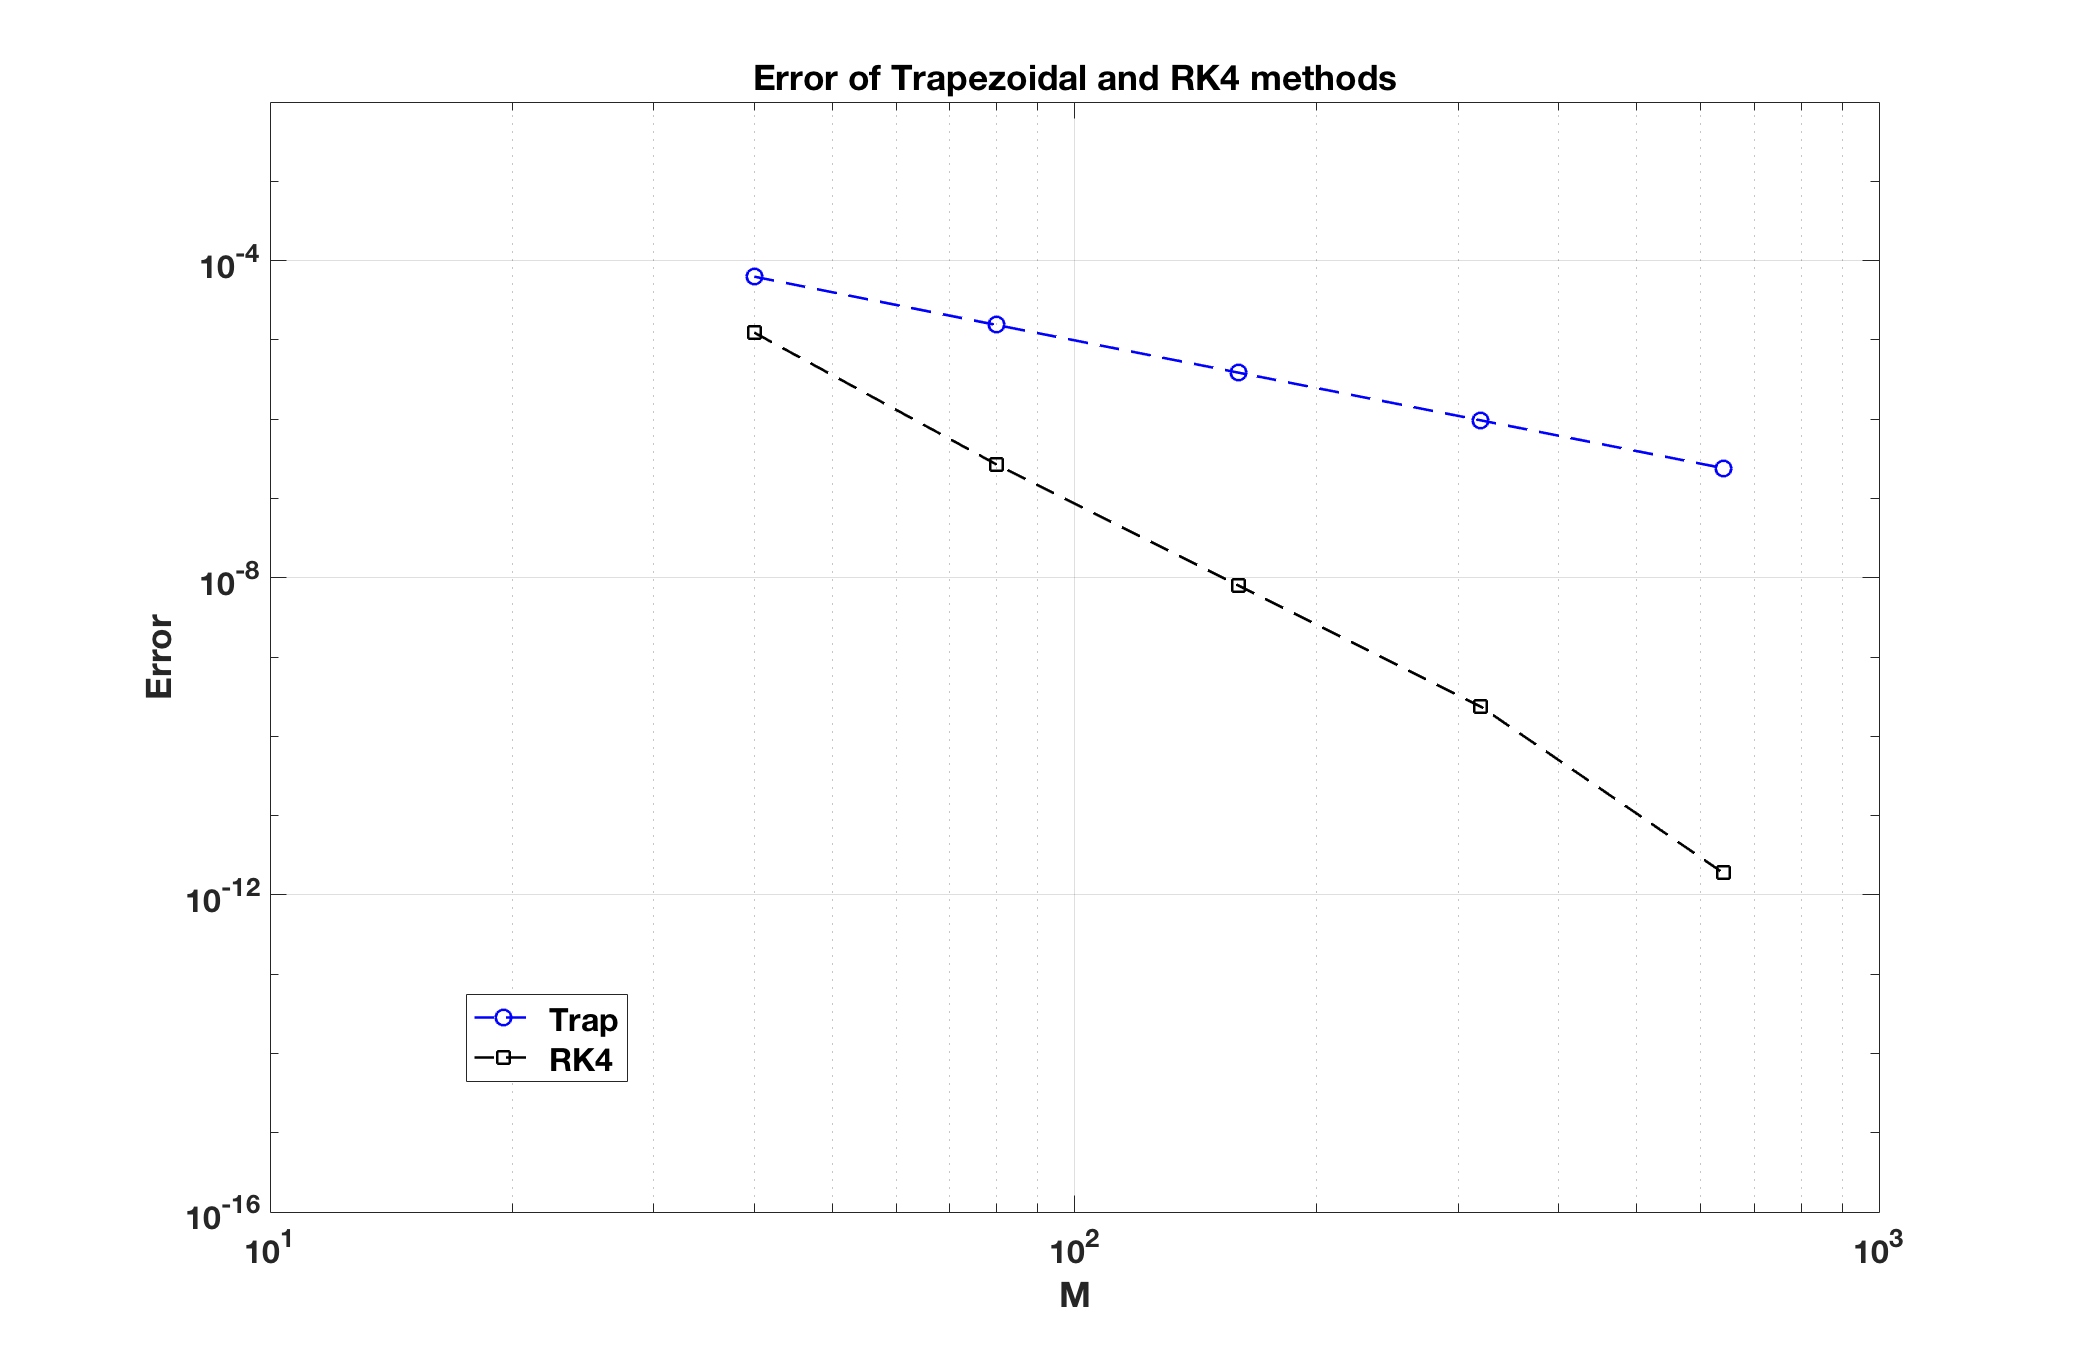
\includegraphics[width=\textwidth]{d.png}

  \item \textit{Compare the two methods based on your results from parts (b)-(d). This includes ease of use, speed of calculation, accuracy of results, and apparent stability.}

    Both of these methods worked quite well; it's no surprise they're widely used. Both are easy to code, though if you don't have the extra thirty seconds to write out the trapezoidal method, RK4 takes a few less lines---anyway, both are easy to use. Both are also quite accurate, with the error reducing quickly to acceptable levels as $M$ increases. However, RK4 again has the edge. RK4 does not outperform trapezoidal method on time consumed. For all values of $M$ used, RK4 took longer to compute than trapezoidal method. Of course, the time taken was still quite small for both methods. Unfortunately, RK4 method was not especially stable for low $M$, while trapezoidal managed to approach the solution even at $M=20$. RK4 of course became stable and won out as $M$ increased, and practically speaking, greater $M$ values will be necessary to achieve the desired accuracy of calculation.


\end{enumerate}












\end{document}
